% Options for packages loaded elsewhere
\PassOptionsToPackage{unicode}{hyperref}
\PassOptionsToPackage{hyphens}{url}
\PassOptionsToPackage{dvipsnames,svgnames,x11names}{xcolor}
%
\documentclass[
  12pt,
  letterpaper,
  DIV=11,
  numbers=noendperiod]{scrartcl}

\usepackage{amsmath,amssymb}
\usepackage{iftex}
\ifPDFTeX
  \usepackage[T1]{fontenc}
  \usepackage[utf8]{inputenc}
  \usepackage{textcomp} % provide euro and other symbols
\else % if luatex or xetex
  \usepackage{unicode-math}
  \defaultfontfeatures{Scale=MatchLowercase}
  \defaultfontfeatures[\rmfamily]{Ligatures=TeX,Scale=1}
\fi
\usepackage{lmodern}
\ifPDFTeX\else  
    % xetex/luatex font selection
\fi
% Use upquote if available, for straight quotes in verbatim environments
\IfFileExists{upquote.sty}{\usepackage{upquote}}{}
\IfFileExists{microtype.sty}{% use microtype if available
  \usepackage[]{microtype}
  \UseMicrotypeSet[protrusion]{basicmath} % disable protrusion for tt fonts
}{}
\makeatletter
\@ifundefined{KOMAClassName}{% if non-KOMA class
  \IfFileExists{parskip.sty}{%
    \usepackage{parskip}
  }{% else
    \setlength{\parindent}{0pt}
    \setlength{\parskip}{6pt plus 2pt minus 1pt}}
}{% if KOMA class
  \KOMAoptions{parskip=half}}
\makeatother
\usepackage{xcolor}
\usepackage[lmargin=0.8in,rmargin=0.8in,tmargin=0.8in,bmargin=0.8in]{geometry}
\setlength{\emergencystretch}{3em} % prevent overfull lines
\setcounter{secnumdepth}{-\maxdimen} % remove section numbering
% Make \paragraph and \subparagraph free-standing
\makeatletter
\ifx\paragraph\undefined\else
  \let\oldparagraph\paragraph
  \renewcommand{\paragraph}{
    \@ifstar
      \xxxParagraphStar
      \xxxParagraphNoStar
  }
  \newcommand{\xxxParagraphStar}[1]{\oldparagraph*{#1}\mbox{}}
  \newcommand{\xxxParagraphNoStar}[1]{\oldparagraph{#1}\mbox{}}
\fi
\ifx\subparagraph\undefined\else
  \let\oldsubparagraph\subparagraph
  \renewcommand{\subparagraph}{
    \@ifstar
      \xxxSubParagraphStar
      \xxxSubParagraphNoStar
  }
  \newcommand{\xxxSubParagraphStar}[1]{\oldsubparagraph*{#1}\mbox{}}
  \newcommand{\xxxSubParagraphNoStar}[1]{\oldsubparagraph{#1}\mbox{}}
\fi
\makeatother


\providecommand{\tightlist}{%
  \setlength{\itemsep}{0pt}\setlength{\parskip}{0pt}}\usepackage{longtable,booktabs,array}
\usepackage{calc} % for calculating minipage widths
% Correct order of tables after \paragraph or \subparagraph
\usepackage{etoolbox}
\makeatletter
\patchcmd\longtable{\par}{\if@noskipsec\mbox{}\fi\par}{}{}
\makeatother
% Allow footnotes in longtable head/foot
\IfFileExists{footnotehyper.sty}{\usepackage{footnotehyper}}{\usepackage{footnote}}
\makesavenoteenv{longtable}
\usepackage{graphicx}
\makeatletter
\def\maxwidth{\ifdim\Gin@nat@width>\linewidth\linewidth\else\Gin@nat@width\fi}
\def\maxheight{\ifdim\Gin@nat@height>\textheight\textheight\else\Gin@nat@height\fi}
\makeatother
% Scale images if necessary, so that they will not overflow the page
% margins by default, and it is still possible to overwrite the defaults
% using explicit options in \includegraphics[width, height, ...]{}
\setkeys{Gin}{width=\maxwidth,height=\maxheight,keepaspectratio}
% Set default figure placement to htbp
\makeatletter
\def\fps@figure{htbp}
\makeatother

%%%%%%%%%%%%%%%%%%%
% Packages/Macros %
%%%%%%%%%%%%%%%%%%%
\usepackage{amssymb,latexsym,amsmath}     % Standard packages

\usepackage{graphicx}
\usepackage[colorlinks=true, allcolors=blue]{hyperref}

\usepackage[round,authoryear]{natbib}
\bibliographystyle{plainnat}
\usepackage{bookmark}

\usepackage{tikz}
\usepackage{tocloft}

\usepackage{placeins}

%%%%%%%%%%%
% Margins %
%%%%%%%%%%%
\KOMAoption{captions}{tableheading}
\makeatletter
\@ifpackageloaded{caption}{}{\usepackage{caption}}
\AtBeginDocument{%
\ifdefined\contentsname
  \renewcommand*\contentsname{Table of contents}
\else
  \newcommand\contentsname{Table of contents}
\fi
\ifdefined\listfigurename
  \renewcommand*\listfigurename{List of Figures}
\else
  \newcommand\listfigurename{List of Figures}
\fi
\ifdefined\listtablename
  \renewcommand*\listtablename{List of Tables}
\else
  \newcommand\listtablename{List of Tables}
\fi
\ifdefined\figurename
  \renewcommand*\figurename{Figure}
\else
  \newcommand\figurename{Figure}
\fi
\ifdefined\tablename
  \renewcommand*\tablename{Table}
\else
  \newcommand\tablename{Table}
\fi
}
\@ifpackageloaded{float}{}{\usepackage{float}}
\floatstyle{ruled}
\@ifundefined{c@chapter}{\newfloat{codelisting}{h}{lop}}{\newfloat{codelisting}{h}{lop}[chapter]}
\floatname{codelisting}{Listing}
\newcommand*\listoflistings{\listof{codelisting}{List of Listings}}
\makeatother
\makeatletter
\makeatother
\makeatletter
\@ifpackageloaded{caption}{}{\usepackage{caption}}
\@ifpackageloaded{subcaption}{}{\usepackage{subcaption}}
\makeatother
\makeatletter
\@ifpackageloaded{tcolorbox}{}{\usepackage[skins,breakable]{tcolorbox}}
\makeatother
\makeatletter
\@ifundefined{shadecolor}{\definecolor{shadecolor}{rgb}{.97, .97, .97}}{}
\makeatother
\makeatletter
\makeatother
\makeatletter
\ifdefined\Shaded\renewenvironment{Shaded}{\begin{tcolorbox}[boxrule=0pt, sharp corners, interior hidden, frame hidden, enhanced, breakable]}{\end{tcolorbox}}\fi
\makeatother

\ifLuaTeX
  \usepackage{selnolig}  % disable illegal ligatures
\fi
\usepackage[round,authoryear]{natbib}
\bibliographystyle{plainnat}
\usepackage{bookmark}

\IfFileExists{xurl.sty}{\usepackage{xurl}}{} % add URL line breaks if available
\urlstyle{same} % disable monospaced font for URLs
\hypersetup{
  pdftitle={Sample File},
  pdfauthor={Gosha Syunyaev},
  colorlinks=true,
  linkcolor={blue},
  filecolor={Maroon},
  citecolor={Blue},
  urlcolor={Blue},
  pdfcreator={LaTeX via pandoc}}


\title{Sample \LaTeX File}
\author{Gosha Syunyaev}
\date{2024-10-25}

\begin{document}
\maketitle


\section{Introduction}

Your introduction goes here! Simply start writing your document and use
the Recompile button to view the updated PDF preview. Examples of
commonly used commands and features are listed below, to help you get
started.

Once you're familiar with the editor, you can find various project
setting in the Overleaf menu, accessed via the button in the very top
left of the editor. To view tutorials, user guides, and further
documentation, please visit our
\href{https://www.overleaf.com/learn}{help library}, or head to our
plans page to
\href{https://www.overleaf.com/user/subscription/plans}{choose your plan}.

\section{Some examples to get started}

\subsection{How to create Sections and Subsections}

Simply use the section and subsection commands, as in this example
document! With Overleaf, all the formatting and numbering is handled
automatically according to the template you've chosen. If you're using
Rich Text mode, you can also create new section and subsections via the
buttons in the editor toolbar.

\subsection{How to include Figures}

First you have to upload the image file from your computer using the
upload link in the file-tree menu. Then use the includegraphics command
to include it in your document. Use the figure environment and the
caption command to add a number and a caption to your figure. See the
code for Figure \ref{fig:frog} in this section for an example.

Note that your figure will automatically be placed in the most
appropriate place for it, given the surrounding text and taking into
account other figures or tables that may be close by.

\begin{figure}
\centering
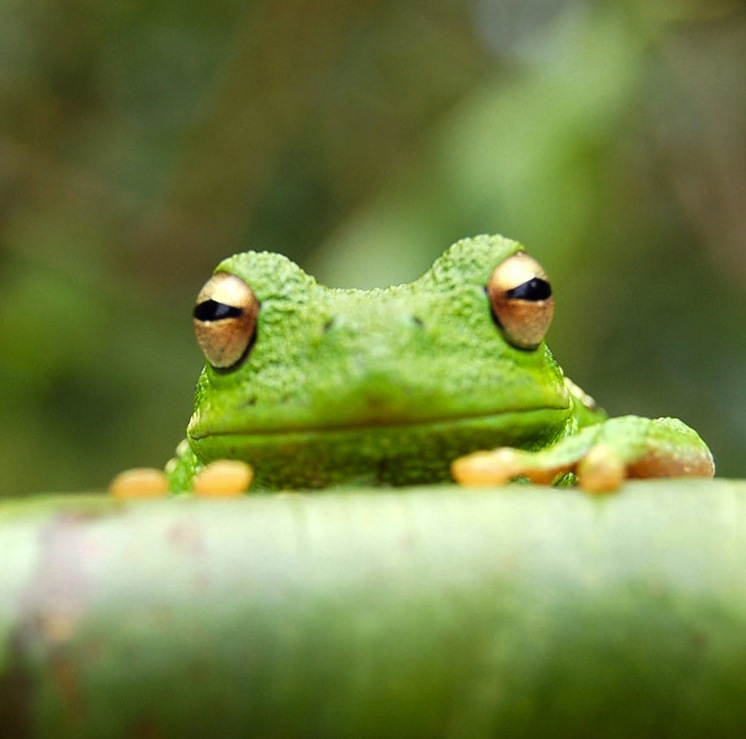
\includegraphics[width=0.3\textwidth]{supp/frog.jpg}
\caption{\label{fig:frog}This frog was uploaded via the file-tree menu.}
\end{figure}

\subsection{How to add Tables}

Use the table and tabular environments for basic tables --- see
Table\textasciitilde{}\ref{tab:widgets}, for example. For more
information, please see this help article on
\href{https://www.overleaf.com/learn/latex/tables}{tables}.

\begin{table}
\centering
\begin{tabular}{l|r}
Item & Quantity \\\hline
Widgets & 42 \\
Gadgets & 13
\end{tabular}
\caption{An example table.}
\end{table}

\subsection{How to add Lists}

You can make lists with automatic numbering \dots

\begin{enumerate}
  \item Like this,
  \item and like this.
\end{enumerate}

\dots or bullet points \dots

\begin{itemize}
  \item Like this,
  \item and like this.
\end{itemize}

\subsection{How to write Mathematics}

\LaTeX{} is great at typesetting mathematics. Let
\(X_1, X_2, \ldots, X_n\) be a sequence of independent and identically
distributed random variables with

\(\text{E}[X_i] = \mu\) and \(\text{Var}[X_i] = \sigma^2 < \infty\), and
let
\[S_n = \frac{X_1 + X_2 + \cdots + X_n}{n} = \frac{1}{n}\sum_{i}^{n} X_i\]

denote their mean. Then as \(n\) approaches infinity, the random
variables \(\sqrt{n}(S_n - \mu)\) converge in distribution to a normal
\(\mathcal{N}(0, \sigma^2)\).

\subsection{How to add Citations and a References List}

You can simply upload a \verb|.bib| file containing your BibTeX entries,
created with a tool such as JabRef. You can then cite entries from it,
like this: \cite{greenwade93}. Just remember to specify a bibliography
style, as well as the filename of the \verb|.bib|. You can find a
\href{https://www.overleaf.com/help/97-how-to-include-a-bibliography-using-bibtex}{video tutorial here}
to learn more about BibTeX.

If you have an
\href{https://www.overleaf.com/user/subscription/plans}{upgraded account},
you can also import your Mendeley or Zotero library directly as a
\verb|.bib| file, via the upload menu in the file-tree.

\begin{verbatim}
Error: object 'countries' not found
\end{verbatim}

\begin{verbatim}
Error in `ggplot()`:
! `data` cannot be a function.
i Have you misspelled the `data` argument in `ggplot()`
\end{verbatim}

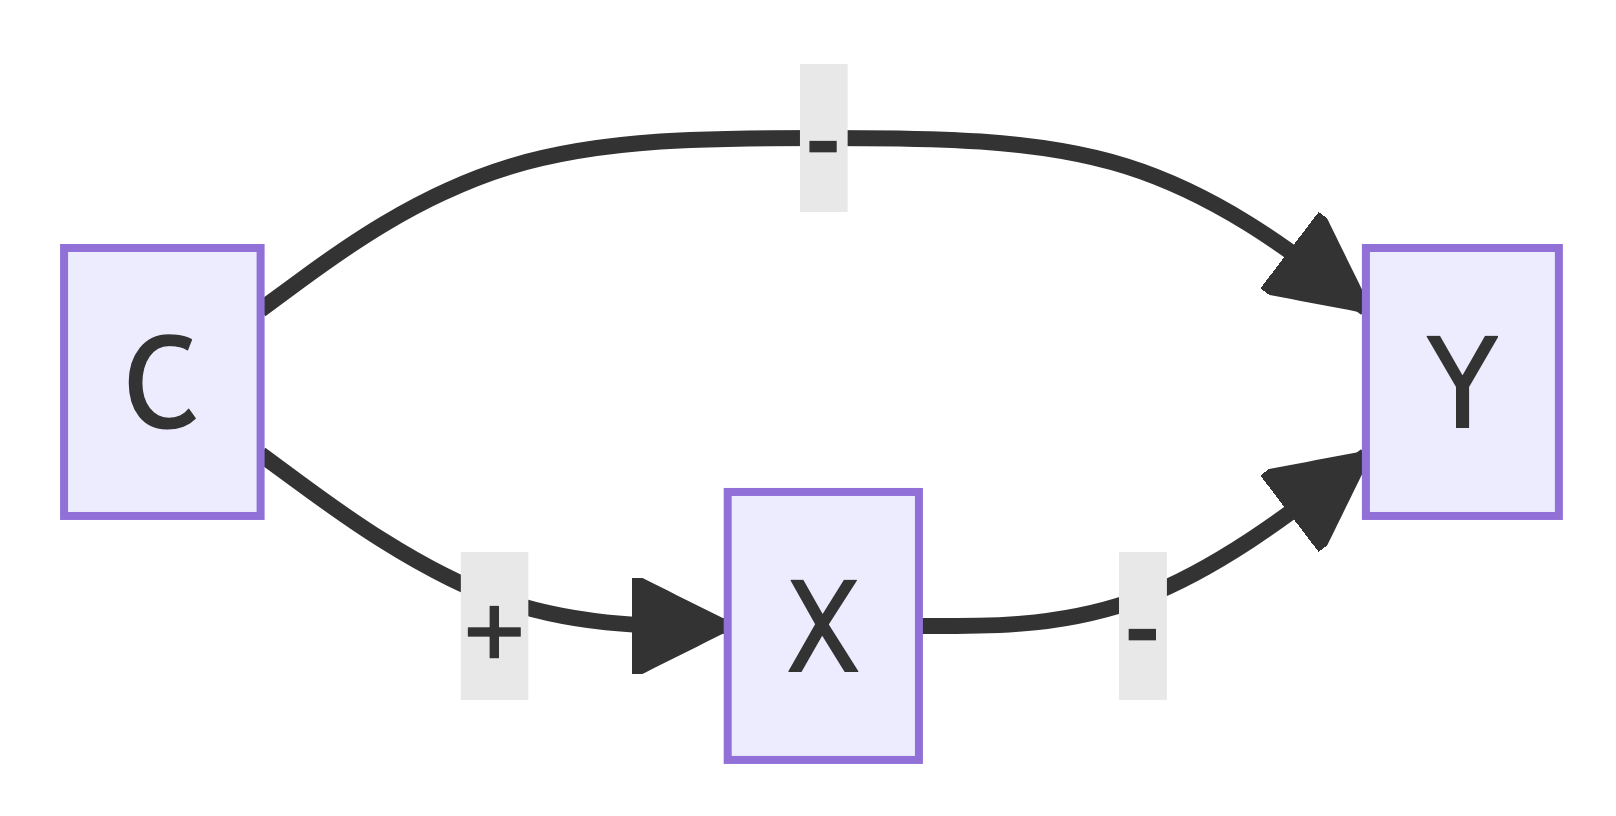
\includegraphics[width=2.11in,height=1.07in]{example_files/figure-latex/mermaid-figure-1.png}


  \bibliography{learning\_bias.bib}



\end{document}
